%\documentclass{cumcmthesis}
\documentclass[withoutpreface,bwprint]{cumcmthesis} %去掉封面与编号页

    \title{“拍照赚钱”APP的定价模型}
    \tihao{A}            % 题号
    \baominghao{042}    % 报名号
    \schoolname{武汉大学}
    \membera{周澳}
    \memberb{傅宇千}
    \memberc{刘志豪}
    \supervisor{指导老师}
    \yearinput{2020}     % 年
    \monthinput{08}      % 月
    \dayinput{21}        % 日

\begin{document}
\maketitle
\begin{abstract}
    “拍照赚钱”APP是。

    \keywords{劳务众包\quad  聚类分析\quad   灰色关联矩阵\quad   多目标优化\quad  }
\end{abstract}
%\tableofcontents
\section{问题重述}
“拍照赚钱”APP是一种基于移动互联网的自助式劳务众包平台,为企业提供各种商业检查和信息搜集服务。用户注册成为APP的会员,然后从APP上领取需要拍照的任务,赚取任务标定的酬金。APP中的任务定价是其运行的核心要素,如果定价不合理,有的任务就会无人问津,而导致商品检查的失败。

附件一是一个已结束项目的任务数据,包含了每个任务的位置、定价和完成情况(“1”表示完成,“0”表示未完成);附件二是会员信息数据,包含了会员的位置、信誉值、参考其信誉给出的任务开始预订时间和预订限额,原则上会员信誉越高,越优先开始挑选任务,其配额也就越大(任务分配时实际上是根据预订限额所占比例进行配发);附件三是一个新的检查项目任务数据,只有任务的位置信息。根据以上内容提出如下四个问题:

\begin{enumerate}
    \item 研究附件一中项目的任务定价规律,分析任务未完成的原因。
    \item 为附件一中的项目设计新的任务定价方案,并和原方案进行比较。
    \item 实际情况下,多个任务可能因为位置比较集中,导致用户会争相选择,一种考虑是将这些任务联合在一起打包发布。在这种考虑下,如何修改前面的定价模型,对最终的任务完成情况又有什么影响?
    \item 对附件三中的新项目给出你的任务定价方案,并评价该方案的实施效果。
\end{enumerate}

\section{符号说明}
\begin{center}
    \begin{tabular}{cc}
        \hline
        \makebox[0.3\textwidth][c]{符号} & \makebox[0.4\textwidth][c]{意义}        \\ \hline
        $cp_k$       &  第$k$名会员的任务完成能力  \\ \hline
        $\overline{cp_i}$       &   第$i$项任务所在网格内会员平均完成能力   \\ \hline
        $p_i$       &  第$i$个任务的定价    \\ \hline
        $C_i$       &   第$i$个任务是否被完成的0-1变量   \\ \hline
        $w_{ij}$       &   任务$i$对会员$j$的吸引度   \\ \hline
        $l_{ij}$       &   任务$i$与会员$j$之间的距离   \\ \hline
        $choice(j)$       &   会员$j$在预定任务时的选择   \\ \hline
        $belong(k)$       &  完成第$k$个任务的会员    \\ \hline
        $G_j$       &  会员$j$的信誉值    \\ \hline
        注:未列出及重复的符号以出现出为准
    \end{tabular}
\end{center}

\section{模型假设}
\begin{enumerate}
    \item 每个任务的工作量基本相同
    \item 会员成功预定的任务都会完成
\end{enumerate}

\section{问题一的建模与求解}

\subsection{问题一的分析}
问题一要求研究已经完成项目中的任务定价规律,并分析其中有大量问完成任务的原因。附件一给出的项目属于结果已经确定的问题,我们需要根据每个任务的定价信息与相关影响因子进行统计分析,从而建立该项目中任务的定价规律。根据经济学原理,市场上一种服务的价格与服务含有的劳动和供求关系有关;本题的数据中能构成对价格的影响因子有任务的位置、任务分布的密度、会员的位置、会员的信誉配额。其中任务与会员的距离和完成任务付出的劳动有关,会员配额、会员和任务的分布密度与供求关系有关。对于“拍照赚钱”的劳务服务,如果假设每个任务的拍照所需的劳动量大致相同,那么会员做不同的任务付出多少的区别便主要来自会员到达任务地点路程远近。对于供求关系,这应当是一个区域性的因素,也就是一个任务的定价受到的供求关系影响主要来自其周边区域,因此我们可以用任务所在区域的任务数密度、会员数密度和会员的信誉值和工作能力来反映。根据以上分析,我们提出以下四种影响任务定价的因素:任务位置、任务所在区域的任务密度,任务所在区域的会员密度,任务所在区域会员的完成能力。通过相关性分析,我们可以得到这些因素与任务定价之间的规律。再通过计算完成的任务与未完成的任务的相关度矩阵的差别,可以分析出一些任务未被完成的原因。

\subsection{建模前的数据分析}
我们首先使用Global Mapper软件把已完成的项目中的每个任务用散点图标注在地图上,用户的位置也同样标注,如下图(红色为未完成任务,绿色为已完成的任务,黄色为用户)

\centerline{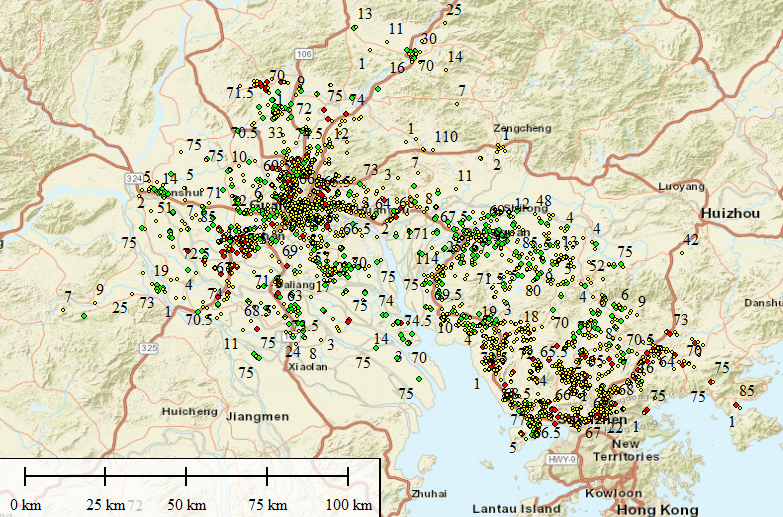
\includegraphics[width=15cm]{1.png}}
可以发现,任务和用户在城市和道路旁较为集中,其他地方较为分散,主要集中在广州、佛山、东莞、深圳等城市。也有几个用户的地理位置远远超出有任务的区域,应当进行去除。

我们把任务对应的定价在散点图上进行了标注,我们通过观察发现,越靠近城市繁华地带,任务和用户越密集,任务的定价也越低。我们猜想这是由于城市内交通便利,用户劳动成本低,同时用户数量多,供给过剩,因此定价低,这是与上节的分析相一致的。为了刻画任务位置对定价的影响,我们认为可以通过选定若干任务的分布中心,通过任务点位置与中心的距离远近给出定价决策的一部分。求解中心可以使用K-均值聚类分析进行。

\subsection{定价模型的建立}

\subsubsection{数据的网格化处理}
找出已完成项目中任务分布的经纬度边界,记经度区间为$[L_{min},L_{max}]$,记纬度区间为$[B_{min},B_{max}]$,将经纬度各划为50等分,则区域被划分为2500各小区域,每个小区域的经度、纬度跨度为$$\Delta L=\frac{L_{max}-L_{min}}{50},\quad \Delta B=\frac{B_{max}-B_{min}}{50}$$则对于给定的经纬坐标$(L,B)$,其所在的经纬网格的行列数为$$i=\lceil \frac{L-L_{min}}{\Delta L}\rceil,\quad j=\lceil \frac{B-B_{min}}{\Delta B}\rceil$$据此可以得出每个任务所在的网格,以及在此区域内的会员所在的网格。

\subsubsection{影响因子的确定}
根据问题分析,任务的定价有四项影响因子,即任务位置、所在网格的任务数密度、所在网格的会员数密度、所在网格的会员完成任务的能力。我们对其具体定义如下:
\begin{enumerate}
    \item 任务所在位置距离其聚类中心的距离$R_i$

    由问题分析中的描述,越接近道路和城市中心,任务定价也就越低,我们通过使用K-均值聚类分析把所有的任务分为若干组,每组有一个中心点,用任务距离中心点的距离$R_i$作为影响定价决策的一个因子,且它们之间是正相关的关系。
    \item 任务所在网格的任务数量$q_i$
    
    对于第$i$项任务,其所在网格内的任务总数记为$q_i$。$q_i$越大,则区域内的服务需求越多,定价与$q_i$应当成正相关关系。
    \item 任务所在网格的会员数量$Q_i$
    
    与上一影响因子相似,网格内会员数量越多,则服务供给越多,定价与$Q_i$应当成负相关关系。
    \item 任务所在网格的会员平均完成能力$\overline{cp_i}$
    
    考虑到每个会员的信誉值、预定限额和开始预定时间各不相同,只考虑会员个数并不能非常准确地反映出区域内地服务供给情况。因此我们提出会员的“任务完成能力”$cp_i$一项指标,信誉值越高、预定限额越大、开始预定时间越早的会员,其完成能力就越大。我们可以通过熵权法,用这些指标得到会员的完成能力。之后便可以计算在每个网格内的会员平均完成能力$\overline{cp_i}$。
\end{enumerate}

\subsubsection{}

\subsection{定价模型的求解}

\subsection{任务未完成原因的分析}

\section{问题二的建模与求解}

\subsection{问题二的分析}
问题一解得的结果仅是已经结束的项目的任务定价模型,问题二进一步要求改进这一项目的定价,这实际上是一个调整定价使APP取得最大效益的优化问题。在APP开发者的角度,高效益应当是付出尽可能少的酬金,完成尽可能多的任务。为了预测项目在某种定价方式下的完成度,我们需要建立会员根据已有的定价选择任务的模型,根据题目的规定和现实生活中的经验,我们提出会员在选择任务时应当遵循以“吸引度”、信誉优先、时间次序的原则,由此可以得到在已知定价的情况下求解任务完成情况的方法。我们可以通过已完成的任务调整模型中的参数,然后可以用这一模型求解定价的优化问题。

\section{问题三的建模与求解}

\section{问题四的建模与求解}

\section{模型总结}

\begin{thebibliography}{9}%宽度9
    \bibitem[1]{1}
    祝胜兰, 饶运清. 一维下料问题的启发式方法[J]. 机械制造与自动化, 2014, 43(001):52-55.
\end{thebibliography}

\begin{appendices}
\end{appendices}
\end{document}